\documentclass[tikz, border=5pt]{standalone}

\begin{document}
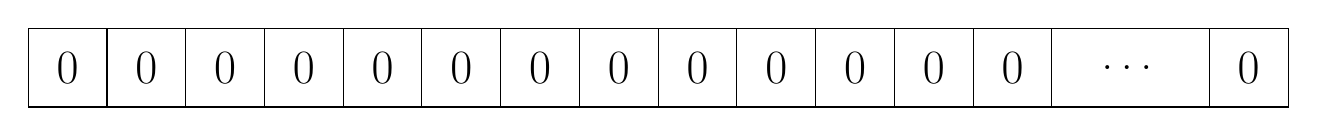
\begin{tikzpicture}

    \foreach \i in {0,...,12} {
            \draw (\i, 0) rectangle (\i + 1, 1);
        }
    \draw (15, 0) rectangle (16, 1);
    \draw (13, 0) rectangle (15, 0);
    \draw (13, 1) rectangle (15, 1);

    \node at (0.5, 0.5) {\LARGE 0};
    \node at (1.5, 0.5) {\LARGE 0};
    \node at (2.5, 0.5) {\LARGE 0};
    \node at (3.5, 0.5) {\LARGE 0};
    \node at (4.5, 0.5) {\LARGE 0};
    \node at (5.5, 0.5) {\LARGE 0};
    \node at (6.5, 0.5) {\LARGE 0};
    \node at (7.5, 0.5) {\LARGE 0};
    \node at (8.5, 0.5) {\LARGE 0};
    \node at (9.5, 0.5) {\LARGE 0};
    \node at (10.5, 0.5) {\LARGE 0};
    \node at (11.5, 0.5) {\LARGE 0};
    \node at (12.5, 0.5) {\LARGE 0};
    \node at (14, 0.5) {\LARGE \dots};
    \node at (15.5, 0.5) {\LARGE 0};

\end{tikzpicture}
\end{document}
